\documentclass[12pt, twoside, openright]{report} %fuente a 12pt, formato doble pagina y chapter a la derecha
\raggedbottom % No ajustar el contenido con un salto de pagina

% MÁRGENES: 2,5 cm sup. e inf.; 3 cm izdo. y dcho.
\usepackage[
a4paper,
vmargin=2.5cm,
hmargin=3cm
]{geometry}

% INTERLINEADO: Estrecho (6 ptos./interlineado 1,15) o Moderado (6 ptos./interlineado 1,5)
\renewcommand{\baselinestretch}{1.15}
\parskip=6pt

% DEFINICIÓN DE COLORES para portada y listados de código
\usepackage[table]{xcolor}
\definecolor{azulUC3M}{RGB}{0,0,102}
\definecolor{gray97}{gray}{.97}
\definecolor{gray75}{gray}{.75}
\definecolor{gray45}{gray}{.45}

% Soporte para GENERAR PDF/A
\usepackage[a-1b]{pdfx}

% ENLACES
\usepackage{hyperref}
\hypersetup{colorlinks=true,
	linkcolor=black, % enlaces a partes del documento (p.e. índice) en color negro
	urlcolor=blue} % enlaces a recursos fuera del documento en azul

% Añadir pdfs como partes del documento
\usepackage{pdfpages}
\usepackage{multicol}

% Quitar la indentación de principio de los parrafos
\setlength{\parindent}{0em}

% EXPRESIONES MATEMATICAS
\usepackage{amsmath,amssymb,amsfonts,amsthm}

\usepackage{txfonts} 
\usepackage[T1]{fontenc}
\usepackage[utf8]{inputenc}

% Insertar graficas y fotos
\usepackage{tikz}
\usepackage{pgfplots}

\usepackage[spanish, es-tabla]{babel} 
\usepackage[babel, spanish=spanish]{csquotes}
\AtBeginEnvironment{quote}{\small}

% diseño de PIE DE PÁGINA
\usepackage{fancyhdr}
\pagestyle{fancy}
\fancyhf{}
\renewcommand{\headrulewidth}{0pt}
\fancyfoot[LE,RO]{\thepage}
\fancypagestyle{plain}{\pagestyle{fancy}}

% DISEÑO DE LOS TÍTULOS de las partes del trabajo (capítulos y epígrafes o subcapítulos)
\usepackage{titlesec}
\usepackage{titletoc}
\titleformat{\chapter}[block]
{\large\bfseries\filcenter}
{\thechapter.}
{5pt}
{\MakeUppercase}
{}
\titlespacing{\chapter}{0pt}{0pt}{*3}
\titlecontents{chapter}
[0pt]                                               
{}
{\contentsmargin{0pt}\thecontentslabel.\enspace\uppercase}
{\contentsmargin{0pt}\uppercase}                        
{\titlerule*[.7pc]{.}\contentspage}                 

\titleformat{\section}
{\bfseries}
{\thesection.}
{5pt}
{}
\titlecontents{section}
[5pt]                                               
{}
{\contentsmargin{0pt}\thecontentslabel.\enspace}
{\contentsmargin{0pt}}
{\titlerule*[.7pc]{.}\contentspage}

\titleformat{\subsection}
{\normalsize\bfseries}
{\thesubsection.}
{5pt}
{}
\titlecontents{subsection}
[10pt]                                               
{}
{\contentsmargin{0pt}                          
	\thecontentslabel.\enspace}
{\contentsmargin{0pt}}                        
{\titlerule*[.7pc]{.}\contentspage}  


% DISEÑO DE TABLAS.
\usepackage{multirow} % permite combinar celdas 
\usepackage{caption} % para personalizar el título de tablas y figuras
\usepackage{floatrow} % utilizamos este paquete y sus macros \ttabbox y \ffigbox para alinear los nombres de tablas y figuras de acuerdo con el estilo definido. Para su uso ver archivo de ejemplo 
\usepackage{array} % con este paquete podemos definir en la siguiente línea un nuevo tipo de columna para tablas: ancho personalizado y contenido centrado
\newcolumntype{P}[1]{>{\centering\arraybackslash}p{#1}}
\DeclareCaptionFormat{upper}{#1#2\uppercase{#3}\par}

% Diseño de tabla para ingeniería
\captionsetup[table]{
	format=hang,
	name=Tabla,
	justification=centering,
	labelsep=colon,
	width=.75\linewidth,
	labelfont=small,
	font=small,
}

% DISEÑO DE FIGURAS.
\usepackage{graphicx}
\graphicspath{{img/}} %ruta a la carpeta de imágenes

% Diseño de figuras para ingeniería
\captionsetup[figure]{
	format=hang,
	name=Fig.,
	singlelinecheck=off,
	labelsep=colon,
	labelfont=small,
	font=small		
}

% NOTAS A PIE DE PÁGINA
\usepackage{chngcntr} %para numeración continua de las notas al pie
\counterwithout{footnote}{chapter}

% LISTADOS DE CÓDIGO
% soporte y estilo para listados de código. Más información en https://es.wikibooks.org/wiki/Manual_de_LaTeX/Listados_de_código/Listados_con_listings
\usepackage{listings}

% definimos un estilo de listings
\lstdefinestyle{estilo}{ frame=Ltb,
	framerule=0pt,
	aboveskip=0.5cm,
	framextopmargin=3pt,
	framexbottommargin=3pt,
	framexleftmargin=0.4cm,
	framesep=0pt,
	rulesep=.4pt,
	backgroundcolor=\color{gray97},
	rulesepcolor=\color{black},
	%
	basicstyle=\ttfamily\footnotesize,
	keywordstyle=\bfseries,
	stringstyle=\ttfamily,
	showstringspaces = false,
	commentstyle=\color{gray45},     
	%
	numbers=left,
	numbersep=15pt,
	numberstyle=\tiny,
	numberfirstline = false,
	breaklines=true,
	xleftmargin=\parindent
}

\captionsetup[lstlisting]{font=small, labelsep=period}
% fijamos el estilo a utilizar 
\lstset{style=estilo}
\renewcommand{\lstlistingname}{\uppercase{Código}}

\pgfplotsset{compat=1.17} 
%-------------
%	DOCUMENTO
%-------------

\begin{document}
\pagenumbering{roman} % Se utilizan cifras romanas en la numeración de las páginas previas al cuerpo del trabajo

%----------
%	PORTADA
%----------	
\begin{titlepage}
	\begin{sffamily}
		\color{azulUC3M}
		\begin{center}
			\begin{figure}[H] %incluimos el logotipo de la Universidad
				\makebox[\textwidth][c]{
\includegraphics[width=16cm]{Portada_Logo.png}}
			\end{figure}
			\vspace{2.5cm}
			\begin{Large}
				Grado en Ingeniería Informática\\
				2019-2020\\
				\vspace{2cm}
				\textsl{Apuntes}\\
				\bigskip
			\end{Large}
			{\Huge Teoría de Automatas y Lenguajes Formales}\\
			\vspace*{0.5cm}
			\rule{10.5cm}{0.1mm}\\
			\vspace*{0.9cm}
			{\LARGE Jorge Rodríguez Fraile\footnote{\href{mailto:100405951@alumnos.uc3m.es}{Universidad: 100405951@alumnos.uc3m.es}  |  \href{mailto:jrf1616@gmail.com}{Personal: jrf1616@gmail.com}}}\\
			\vspace*{1cm}
		\end{center}
		\vfill
		\color{black}
		
\includegraphics[width=4.2cm]{img/creativecommons.png}\\
		Esta obra se encuentra sujeta a la licencia Creative Commons\\ \textbf{Reconocimiento - No Comercial - Sin Obra Derivada}
	\end{sffamily}
\end{titlepage}

%----------
%	ÍNDICES
%----------	

%--
% Índice general
%-
\tableofcontents
\thispagestyle{fancy}

%----------
%	TRABAJO
%----------	

\pagenumbering{arabic} % numeración con múmeros arábigos para el resto de la publicación	


%----------
%	COMENZAR A ESCRIBIR AQUI
%----------	


\part{TEMA 1. Introducción}
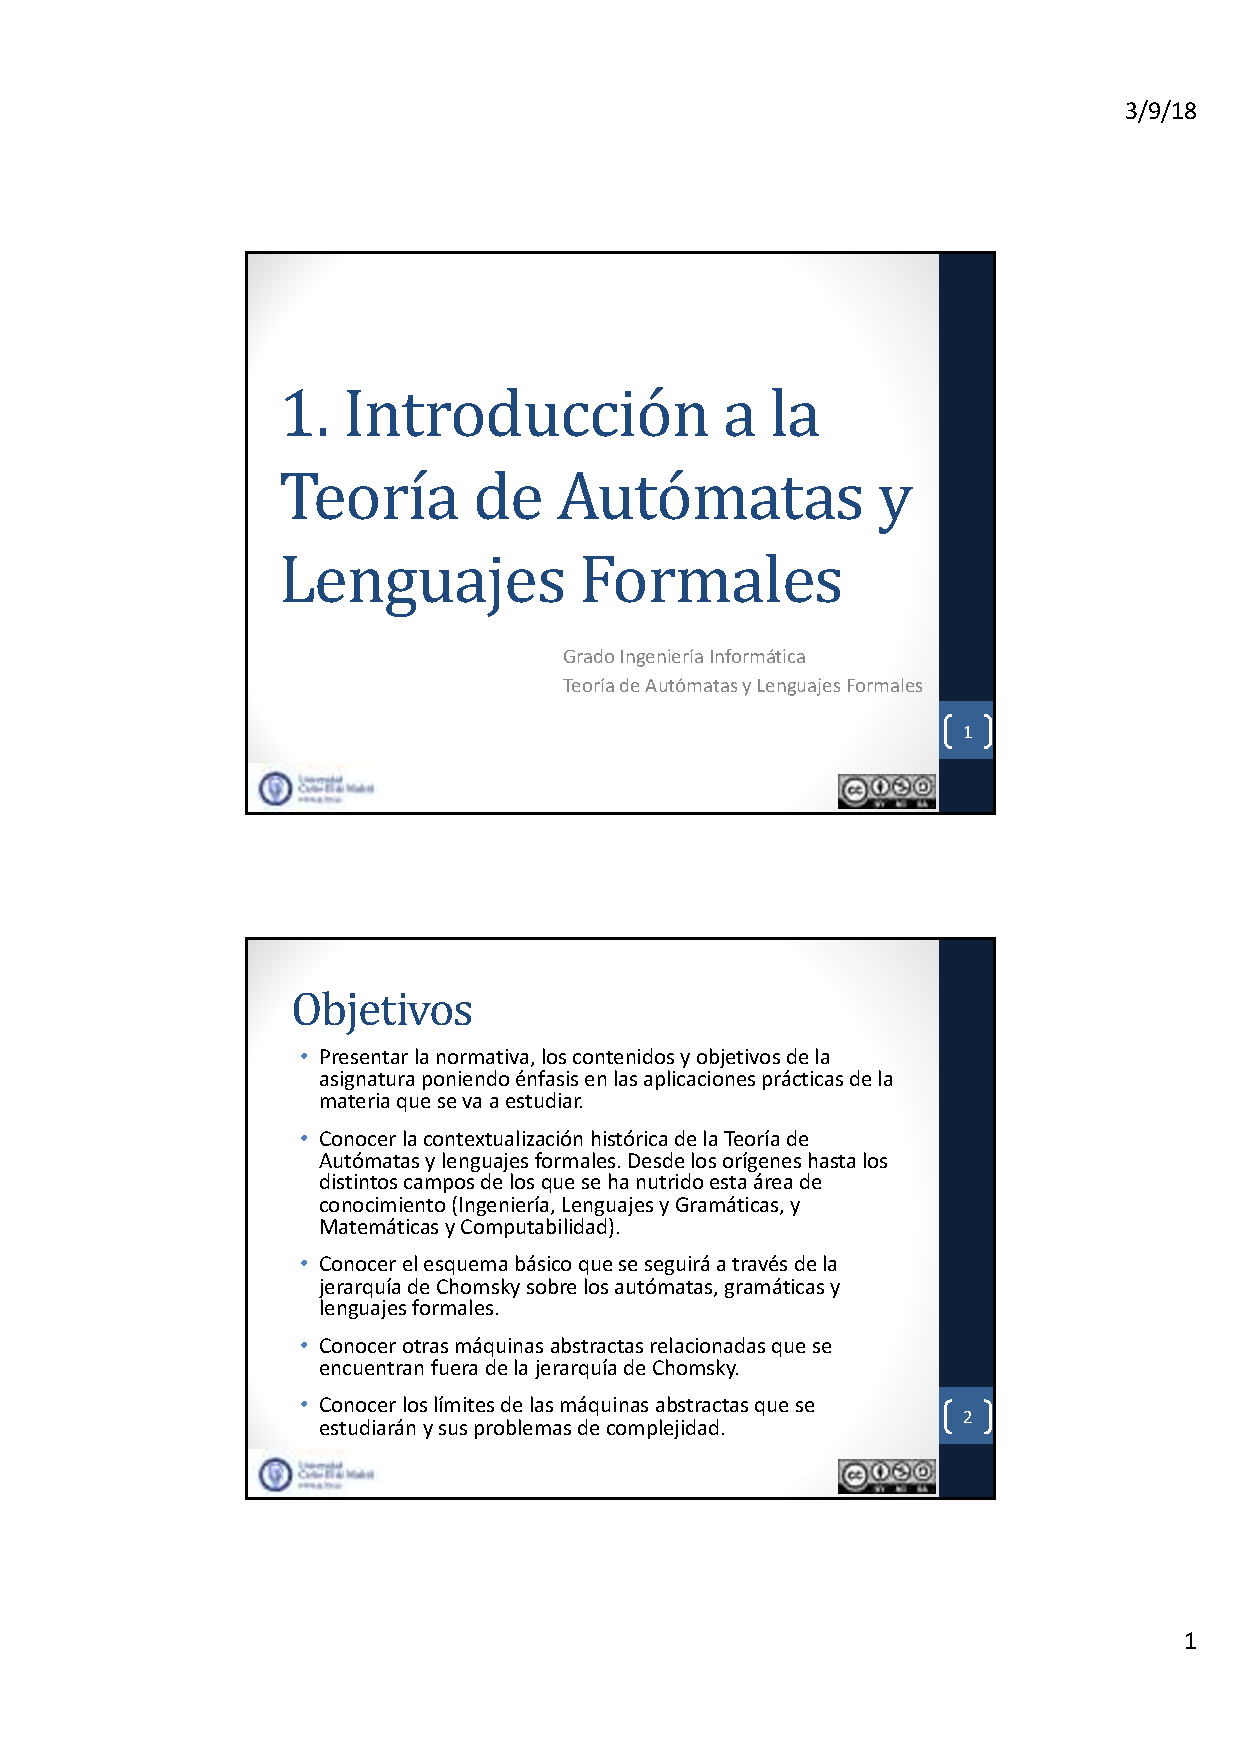
\includepdf[pages=-]{docs/Tema1_TALF.pdf}

\part{TEMA 2. Autómatas Formales}
\includepdf[pages=-]{docs/Tema2-TALF.pdf}

\part{TEMA 3. Autómatas Finitos}
\includepdf[pages=-]{docs/Tema3-TALF_Ampliado.pdf}

\part{TEMA 4. Gramáticas y Lenguajes Formales}
\includepdf[pages=-]{docs/Tema4_TALF.pdf}

\part{TEMA 5. Expresiones Regulares}
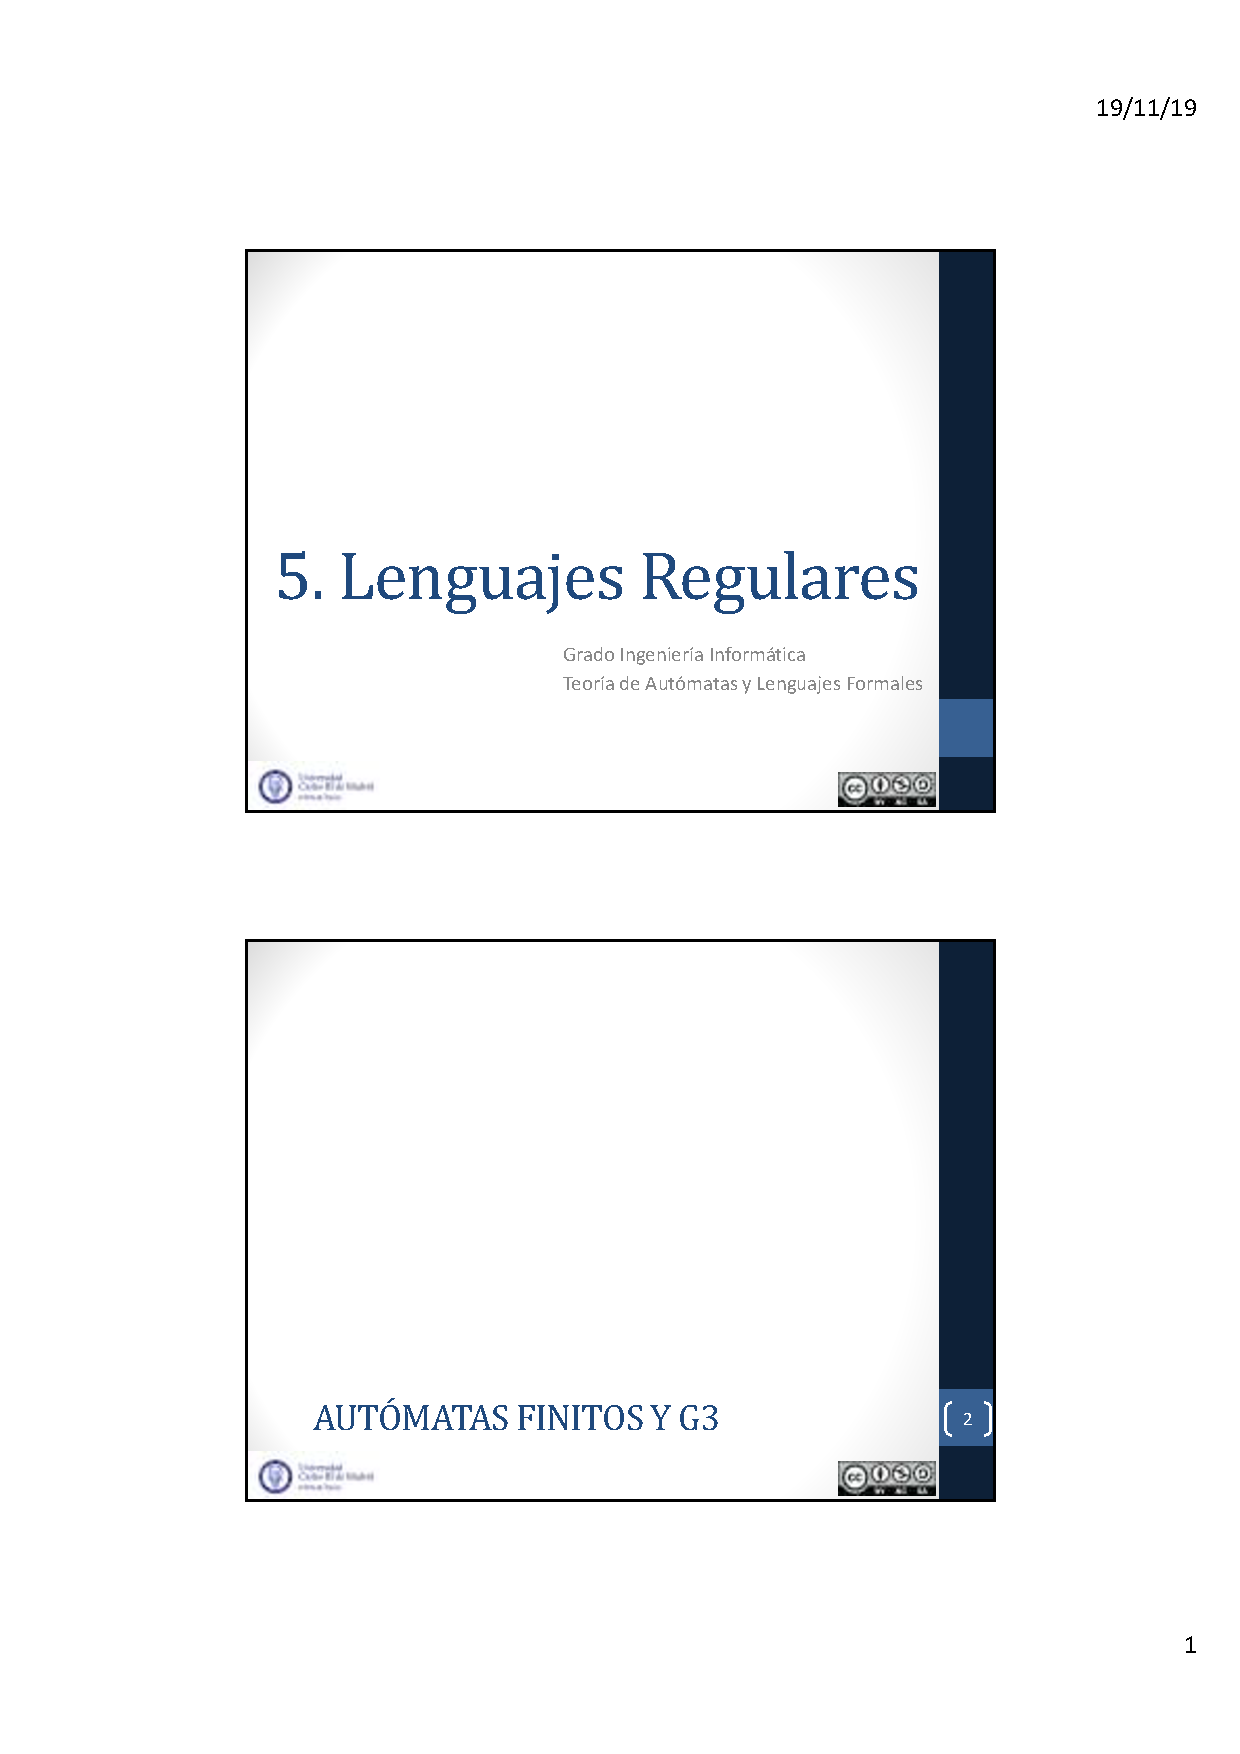
\includepdf[pages=-]{docs/Tema5_TALF_corregido.pdf}
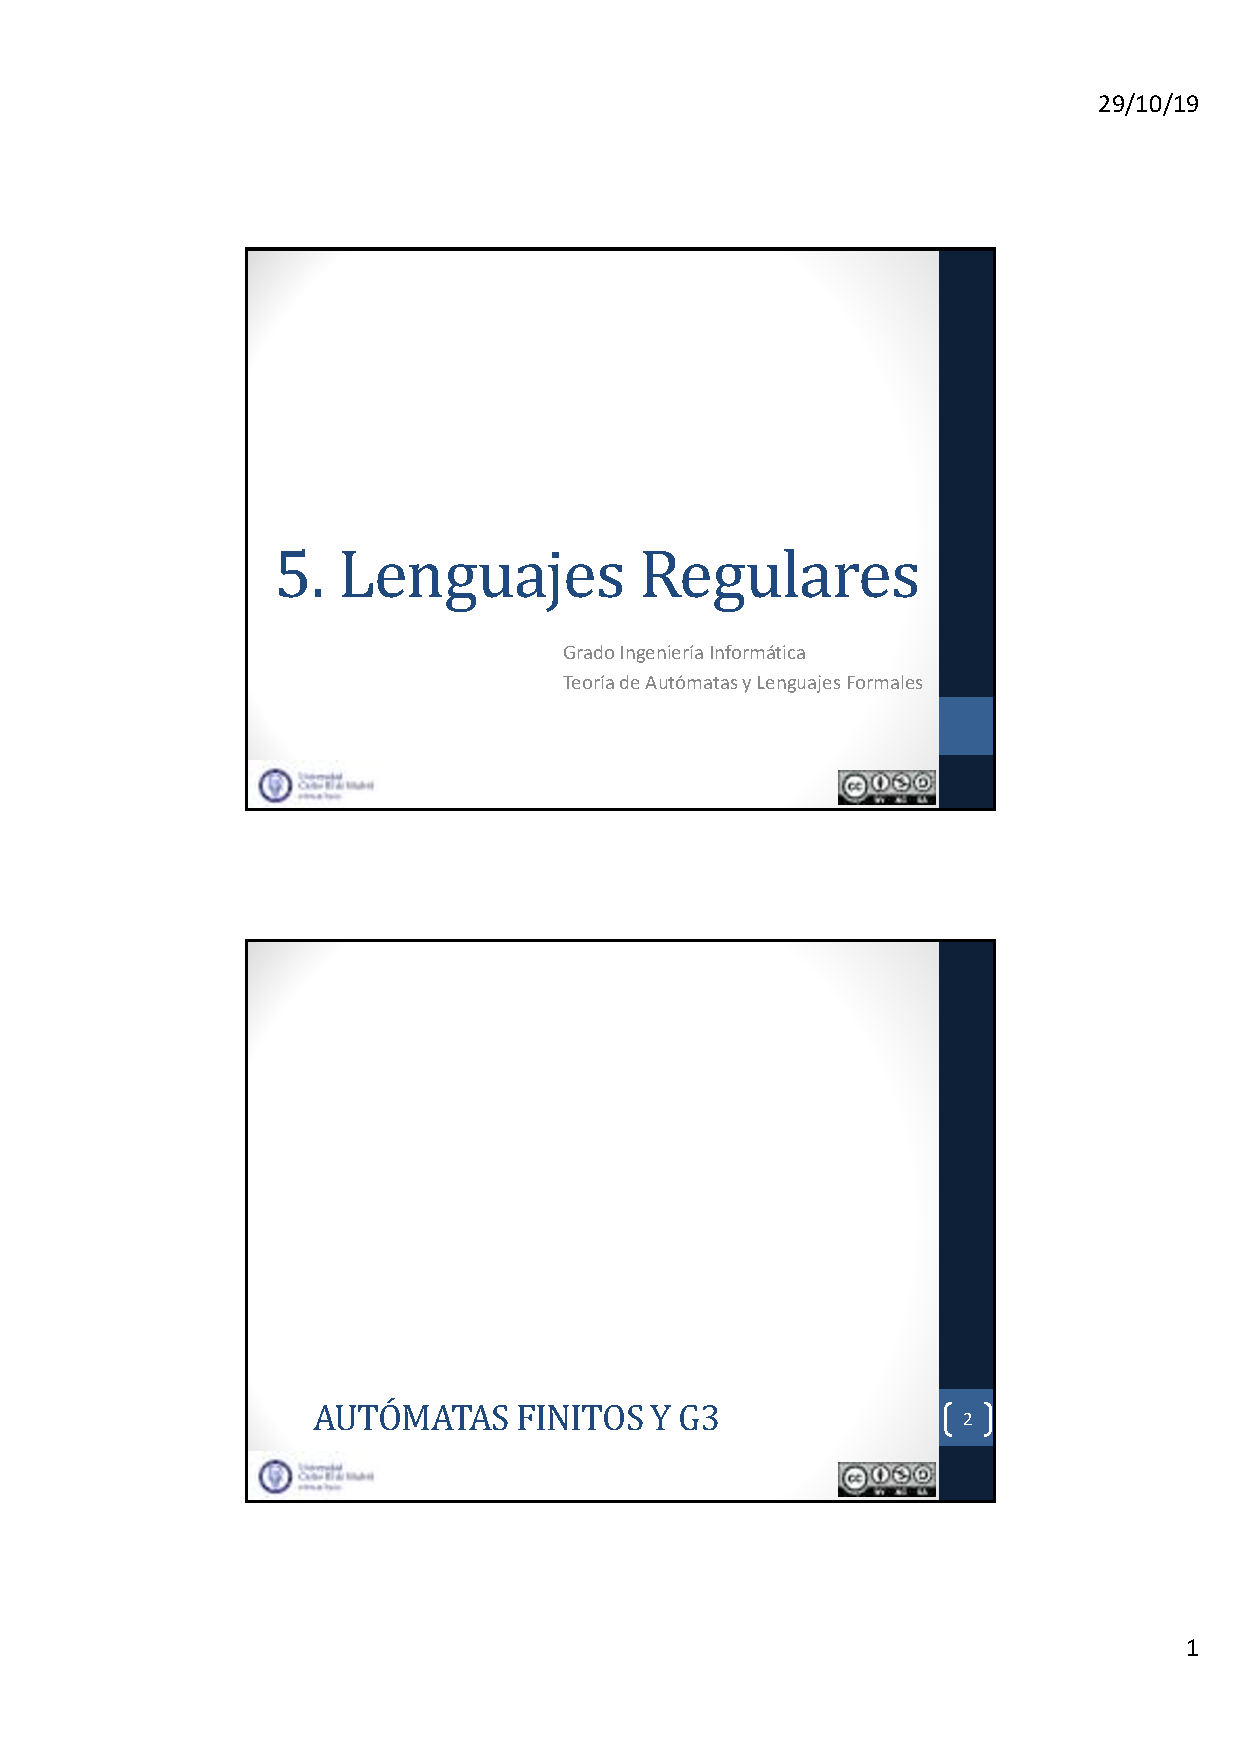
\includepdf[pages=-]{docs/Tema5_TALF.pdf}

\part{TEMA 6. Autómatas a Pila}
\includepdf[pages=-]{docs/Tema6_TALF.pdf}

\part{TEMA 7. Maquina de Turing}
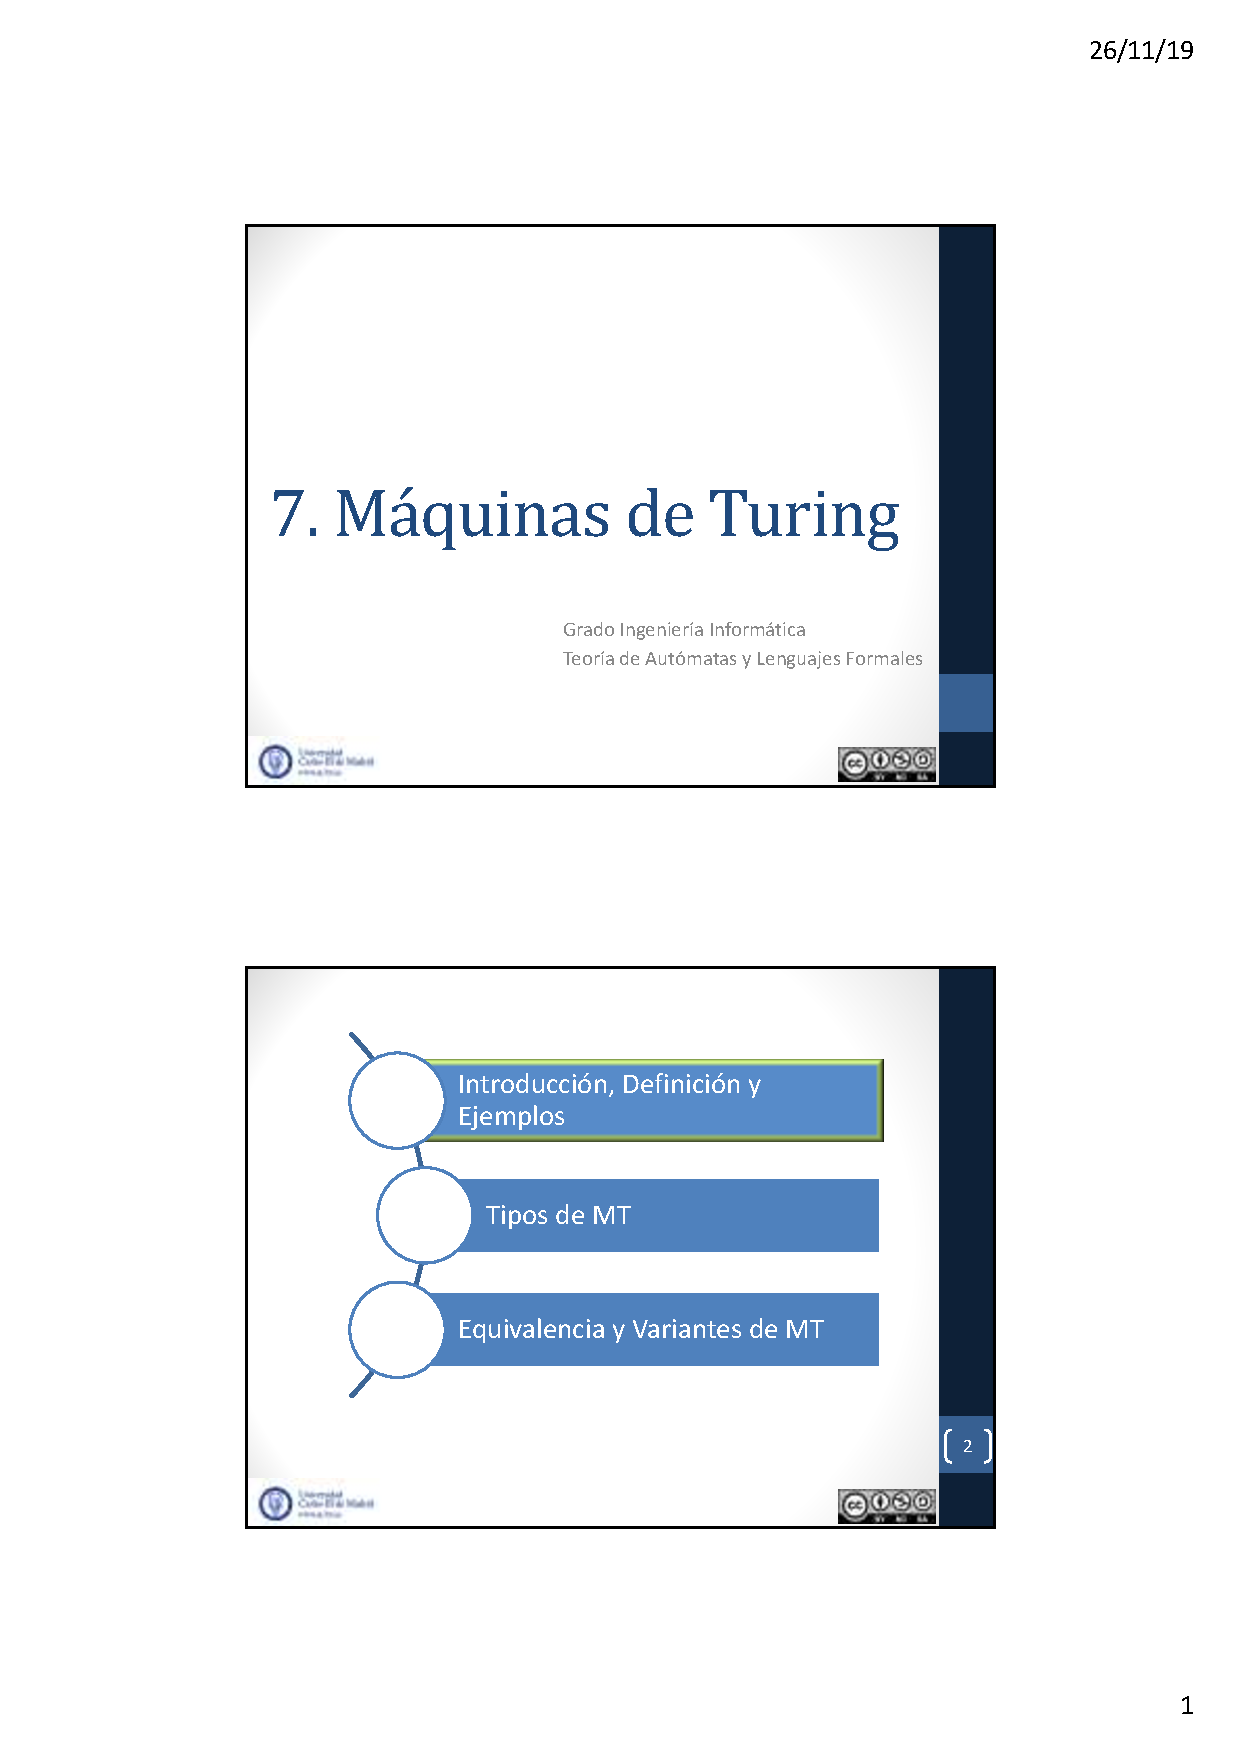
\includepdf[pages=-]{docs/Tema7_TALF_OJO_MODIFICADO.pdf}

\part{TEMA 8. Complejidad Computacional}
\includepdf[pages=-]{docs/Tema8_TALF.pdf}

\chapter{Recursos}
\textbf{Limpiar y bien formar siempre}
\section{Tema 3}
\subsection{$\boldsymbol{AFD \rightarrow AFD} \textit{ mínimo}$}
\begin{enumerate}
	\item Buscar $Q/E_0$, que divide los estados en finales y no finales.
	\item Hacer $Q/E_1, Q/E_2...$ pueden separarse, pero nunca juntarse de nuevo.
	\item Cuando se repitan las particiones hemos terminado. Como máximo tendremos que hacer $Q/E_{(n-2)}$ iteraciones.
\end{enumerate}

\subsection{$\boldsymbol{AFND \rightarrow AFD}$}
\begin{enumerate}
	\item Calcular $T^*$.
	\item Quitar la columna $\lambda$ y añadir la columna $\lambda^*$.
	\item Sustituir la columna a, b… por $\lambda^* a \lambda^*$, $\lambda^* b \lambda^*$...
	\item El nuevo estado inicial será p $\lambda^*$.
	\item Transformar los caminos múltiples en estados combinados (finales si alguna de las letras es final) y las transiciones no definidas en transiciones al sumidero.
\end{enumerate}

\section{Tema 4}
\subsection{$\boldsymbol{\textit{G3 LD} \rightarrow \textit{G3 LI}}$}
\begin{enumerate}
	\item Quitar el axioma inducido ($A \rightarrow aS$) introduciendo un nuevo símbolo (que haga lo mismo que el axioma, pero no se copia lambda)
	\item Construir un grafo dirigido en el que los nodos son los $\Sigma_{NT}$ y las flechas son los $\Sigma_T$.
	\item Intercambiar las etiquetas de $\lambda$ y S, y dar la vuelta a las flechas.
	\item Interpretar el grafo

	      Nota: las que iban de S van a $\lambda$, y de $\lambda$ no puede salir nada.
\end{enumerate}

\subsection{Lenguaje vacío (G2)}
Generar el árbol de derivación hasta llegar a n (número de estados). Si no genera
sentencias y se repiten los $\Sigma_{NT}$, es un lenguaje vacío.

\subsection{Lenguaje infinito (G2)}
Construir un grafo cuyos nodos están etiquetados con los $\Sigma_{NT}$. Si existen ciclos
accesibles desde el axioma, entonces es un lenguaje infinito.

\subsection{Limpieza y bien-formación de gramáticas}
\begin{enumerate}
	\item Eliminar reglas innecesarias ($A \rightarrow A$)
	\item Eliminar símbolos inaccesibles (para ello se construye un vector con los símbolos T y NT)

	      Ir marcando desde el axioma los que vaya produciendo.
	\item Eliminar reglas superfluas con el algoritmo de marcado
	      \begin{enumerate}
		      \item Se marcan los $\Sigma_{NT} \rightarrow \Sigma_{T}$ y los $\Sigma_{NT} \rightarrow \lambda$
		      \item Se marcan los que contengan un $\Sigma_{NT}$ marcado en la derecha
		      \item Se repite hasta que no se pueden marcar más
		      \item Se eliminan todas las reglas no marcadas
	      \end{enumerate}
	\item Eliminar los símbolos no generativos, es decir, aquellos que solo aparecen en reglas superfluas.
	\item Eliminar las reglas no generativas, las de tipo $A \rightarrow \lambda$. Cada vez que aparezca A en la $\lambda$. Se admite parte derecha, se añade la posibilidad de que sea $\textit{Axioma} \rightarrow \lambda$, OJO si cuando eliminamos solo quedaba un símbolo ($C \rightarrow M$ y eliminamos M), ponemos lambda ($C \rightarrow \lambda$) y repetimos el proceso de eliminación (para C).
	\item Eliminar las reglas de redenominación, las de tipo $A \rightarrow B$. Por cada regla de la forma $B \rightarrow x$, se añade $A \rightarrow x$
\end{enumerate}

\subsection{$\boldsymbol{G2 \rightarrow FNC}$}
Se separa el primer símbolo de la derecha del resto, por ejemplo, de $A \rightarrow aBb$ sacamos $A \rightarrow DE$ y $D \rightarrow a$, $E \rightarrow Bb \rightarrow BC$, $C \rightarrow b$ (previo paso debe estar limpia y bien formada)

\subsection{$\boldsymbol{G2 \rightarrow FNG}$}
\begin{enumerate}
	\item Limpiar y bien formar la gramática.
	\item Quitar recursividad a izquierdas si las reglas. $\lambda$ no se toca en este paso
	\item Ordenar el alfabeto $\Sigma_{NT}$ (A, B) y clasificar las reglas en G2(AB) o G3(BA)
	\item Pasar las de G3 a G2. Se hace por sustitución, no sustituir con las reglas que dan $\lambda$
	      \begin{enumerate}
		      \item Quitar recursividad a izquierdas si apareciese.
	      \end{enumerate}
	\item Pasar de G2 a G1, empezando por la que me deje meter un $\Sigma_T$ en la cabeza.
	\item Si hay un $\Sigma_T$ que no esté en la cabeza, sustituirlo por un $\Sigma_{NT}$ que dé ese $\Sigma_T$.
\end{enumerate}

\subsection{Quitar recursividad a izquierdas}
Dada una regla de tipo $A \rightarrow A\alpha \; | \; \beta$ (donde $\alpha$ y $\beta$ son cualquier cosa...)

Se transforma en:
\begin{itemize}
	\item $A \rightarrow \beta \; | \; \beta X$
	\item $X \rightarrow \alpha X \; | \; \alpha$
\end{itemize}
Si tuviéramos varias ($A \rightarrow A\alpha \; | \; \beta_1 \; | \; \beta_2$), entonces se transforma en:
\begin{itemize}
	\item $A \rightarrow \beta \; | \; \beta X$
	\item $X \rightarrow \alpha X \; | \; \alpha$
\end{itemize}

\subsection{Paso de G3LD (FNG) $\boldsymbol{\rightarrow}$ AF y viceversa}
Por cada regla $A \rightarrow aB$:
\begin{itemize}
	\item A y B son estados del autómata y se realiza la transición de A a B con ‘a’.
\end{itemize}
Si tenemos una regla del tipo $A \rightarrow a$:
\begin{itemize}
	\item Se realiza la transición de A a un estado final con ‘a’.
\end{itemize}
Para pasar de AF a G3LD se hace exactamente igual.

\section{Tema 5}
\subsection{Teoria de síntesis}
Nota: $D_{ab}(\alpha)= D_b(D_a(\alpha))$
\begin{enumerate}
	\item Derivar la expresión respecto de todos los símbolos y todas las que me vayan saliendo.

	      Las voy llamando $R_x$, donde x es un Número
	\item Si $R_x$ puede ser $\lambda$, se añade una regla, $R_x \rightarrow \lambda$
	\item Si $D_y(R_{x_1}) = R_{x_2}$, se añade una regla $R_{x_1} \rightarrow y R_{x_2}$
	\item Luego se aplica el paso de G3LD (FNG) a AF para obtener el AF correspondiente
\end{enumerate}
\begin{table}[H]
	\centering\begin{tabular}{ll}
		$D_a(a) = \lambda$ \\
		$D_a(b) = \emptyset$ \\
		$D_a(RS) = D_a(R)S + d(R)D_a(S)$ \\
		$D_a(R+S) = D_a(R) + D_a(S)$ \\
		$D_a(R^*) = D_a(R)R^*$ \\
		$d(a) = \emptyset$ \\
		$d(a^*) = \lambda$ & Si puede ser $\lambda$, es $\lambda$, si no $\emptyset$ \\
		$d(a^*+a) = \lambda$ \\
	\end{tabular}
\end{table}

\section{Tema 6}
\subsection{$\boldsymbol{APF \rightarrow APV}$}
\begin{enumerate}
	\item Añadir un estado inicial nuevo con una transición y un nuevo ''chivato'' que nos indique cuando se vacía la pila
	\item Añadir un estado ''final'' que desapile todo lo que pudiera quedar y el chivato.
\end{enumerate}
\subsection{$\boldsymbol{APV \rightarrow APF}$}
\begin{enumerate}
	\item Añadir un estado inicial nuevo con su chivato
	\item Añadir un estado final al que se transita desapilando el chivato
\end{enumerate}

\subsection{$\boldsymbol{G2 \; (FNG) \rightarrow APV}$}
\begin{enumerate}
	\item Tres tipos de reglas:
	      \begin{enumerate}
		      \item $A \rightarrow aBCD: \; f(q,\; a,\; A) = (q,\; BCD)$
		      \item $A \rightarrow a: \; f(q,\; a,\; A) = (q,\; \lambda)$
		      \item $S \rightarrow \lambda: \; f(q,\; \lambda,\; S) = (q,\; \lambda)$
	      \end{enumerate}
	\item El automata tendrá un único estado, q.
\end{enumerate}

\subsection{$\boldsymbol{APV \rightarrow G2}$}
\begin{enumerate}
	\item Se pone una regla del tipo $S \rightarrow (q_0, \; A_0, \; pqr...)$
	\item Se ponen reglas de tipo:
	      \begin{enumerate}
		      \item Tipo $1A: \; f(q, \; a, \; B) = (p, \; DEF)$

		            El molde será: $(qB\_) \rightarrow a(pD\_)(\_E\_)(\_F\_)$

		      \item Tipo $1B: \; f(p, \; \lambda, \; B) = (q, \; A)$

		            El molde será: $(pB\_) \rightarrow X(qA\_)$

		      \item Tipo $2A: \; f(p, \; a, \; B) = (q, \; \lambda)$

		            El molde será: $(pBq) \rightarrow a$

		      \item Tipo $2B: \; f(p, \; \lambda, \; B) = (q, \; \lambda)$

		            El molde será: $(pBq) \rightarrow \lambda$


	      \end{enumerate}
\end{enumerate}
\pagebreak
\subsection{Equivalencia de EERR}
\begin{multicols}{2}
	\begin{enumerate}
		\item $(\alpha+\beta)+\sigma = \alpha + (\beta + \sigma)$
		\item $\alpha + \beta = \beta + \alpha$
		\item $(\alpha \cdot \beta)\cdot\sigma = \alpha \cdot (\beta\cdot\sigma)$
		\item $\alpha \cdot (\beta +\sigma) = (\alpha \cdot \beta) + (\alpha \cdot \sigma)$

		      $(\beta +\sigma) \cdot \alpha  = (\beta \cdot \alpha) + (\sigma \cdot \alpha)$
		\item $\alpha \cdot \lambda = \lambda \cdot \alpha = \alpha$
		\item $\alpha + \phi = \phi + \alpha = \alpha$
		\item $\lambda^* = \lambda$
		\item $\alpha \cdot \phi = \phi \cdot \alpha= \phi$
		\item $\phi^* = \lambda$
		\item $\alpha^* \cdot \alpha^* = \alpha^*$
		\item $\alpha \cdot \alpha^* = \alpha^* \cdot \alpha$
		      \columnbreak
		\item $(\alpha^*)^*=\alpha^*$
		\item $\alpha^* = \lambda + \alpha + \alpha^2 + ... + \alpha^n + \alpha^{n+1} \cdot \alpha^*$
		\item $\alpha^* = \lambda + \alpha \cdot \alpha^*$
		\item $\alpha^* = (\lambda + \alpha)n-1 + \alpha n \cdot \alpha^*$
		\item Sea $f$ una función, $f: E_{\Sigma^n} \rightarrow E_\Sigma$ se verifica:

		      $f(\alpha, \beta, ..., \sigma) + (\alpha + \beta + ... + \sigma)^* = (\alpha + \beta + ... + \sigma)^*$
		\item Sea $f$ una función, $f: E_{\Sigma^n} \rightarrow E_\Sigma$ se verifica:

		      $(f(\alpha^*, \beta^*, ..., \sigma^*))^* = (\alpha + \beta + ... + \sigma)^*$
		\item $(\alpha^* + \beta^*)^* = (\alpha^* \cdot \beta^*)^* = (\alpha + \beta)^*$
		\item $(\alpha \cdot \beta)^*\cdot \alpha = \alpha \cdot (\beta \cdot \alpha)^*$
		\item $(\alpha^* \cdot \beta)^*\cdot \alpha^* =(\alpha + \beta)^*$
		\item $(\alpha^* \cdot \beta)^*\cdot \alpha^* = \lambda + (\alpha + \beta)^*\cdot \beta$
		\item R. Inferencia: $X=Ax + B \rightarrow X = A^* \cdot B$
	\end{enumerate}
\end{multicols}

\subsection{Analisis}
\begin{enumerate}
	\item Hacer las ecuaciones del Automata Finito

	      De $X_0$ a $X_1$ con una 'a': $X_0 = aX_1$

	      De $X_0$ a $X_2$ que es final con una 'b': $X_0 = b X_2 + b$

	      Si hay varias transiciones se ponen en la misma ecuación sumándose

	      Si el estado final solo va al sumidero o no tiene ramas se le añade $\lambda$

	\item Utilizar las equivalencias de EERR, empezando por las más lejanas al inicial. Esencialmente se usa la regla de inferencia
	      \begin{table}[H]
		      \centering\begin{tabular}{ll}
			      $X_0 = aX_0$     & $X_0 = \emptyset$ \\
			      $X_1 = bX_1 + c$ & $X_1 = b^*c$      \\
			      $X_2 = c$        & $X_2 = c$         \\
		      \end{tabular}
	      \end{table}
\end{enumerate}

\subsection{Formatos}
AFD = (Alfabeto, Q, $q_0$, f, F) F = Estado finales f=Función transición

AFND = (Alfabeto, Q, $q_0$, f, F, T) T = Transiciones con $\lambda$

G = (Terminales, No Terminales, S, P) S = Axioma P = Transiciones

AP = (Alfabeto cinta, Alfabeto pila, Q, $A_0$, $q_0$, f, F)  $A_0$ = Fondo pila

MT = (Alfabeto de entrada, Alfabeto cinta, b, Q, $q_0$, f, F) b = Símbolos especiales

\subsection{Jeraquia de Chomsky}
Todos aceptan axioma para dar $\lambda$

\begin{description}
	\item[G0] Lenguaje sin restricciones, puede ser cualquier cosa, se caracteriza por reglas compresoras ($aVs \rightarrow d$ OJO también si no es axioma $B \rightarrow \lambda$) y estructura de frases ($AS \rightarrow SA$)
	\item[G1] Sensible al contexto, puede ser cualquier cosa, sin reglas compresoras y Contexto ($aS \rightarrow ADC$)
	\item[G2] De contexto libre, un símbolo a la izquierda pero cualquier cosa a la derecha. También si hay G3LD y G3LI en la misma gramática.
	\item[G3] Gramática regular, son las de la forma $NT \rightarrow T$ y un tipo de las siguientes reglas:
	      \begin{table}[H]
		      \centering\begin{tabular}{ll}
			      G3LI & $NT \rightarrow NT \; T$ \\
			      G3LD & $NT \rightarrow T \; NT$
		      \end{tabular}
	      \end{table}
\end{description}

\end{document}